\subsection{From 1D to 2D}
After inspecting the 2D FFT algorithm, we realized that it shows a promising potential for parallelization. The steps for performing 2D FFT are as follows: 
\begin{itemize}
    \item Perform a row-wise FFT on each row of the image (which can be done completely in parallel).
    \item Transpose the image. This stage and the following one could be ommited and be replaced by a column-wise FFT, but since the memory access pattern would not efficient the image is transposed instead.
    \item Perform a row-wise FFT on each row of the transposed image (which are the columns of the original matrix).
    \item Transpose the matrix once again to maintain the original order.
\end{itemize}
It should be clear now that if we consider a \(n * n \) image, n parallel processes can do the required calculations for the row-wise FFTs and then for the column-wise FFT. While some level of parallelism can be achieved with a multi-core CPU, the speedup would not be significant, as the number of cores are limited, hence the need for an accelerator.

\subsection{Moving the calculations to the GPU}
What makes GPUs the perfect candidate for this algorithm is the massive parallelism they can provide because of their large thread count. As an example, the device we used for testing was shipped with an NVIDIA RTX3070 mobile GPU, which offers 5120 CUDA cores, a number that is very impressive considering it is a consumer-grade laptop. With that in mind, we moved 2D FFT computations to the GPU by implementing several CUDA kernels that can be found in \texttt{FFTGPU.cu} and wrappers that can be located in \texttt{FourierTransform.cpp}.
As a first implementation, we implemented each step in a separate kernel, one each for:
\begin{itemize}
    \item bit reversal permutation
    \item 1D FFT
    \item transposition
\end{itemize}

Then, in the wrapper \texttt{IterativeFFTGPU2D}, we would move data from the host (CPU) to the device (GPU) and launch the kernels in the above order. After performing the calculations, we would move the data back to the host. Finally, we would call the wrapper for \texttt{cuda\_main.cpp} and use OpenCV to check the correctness of the results.

\subsection{Block by block FFT}
Since one of our objectives was to perform image compression, we realized that most of the algorithms for compression (including JPEG, which our compression algorithm was deeply inspired by) use 8x8 subblocks instead of performing transformations on the whole input at once. So, with that in mind, another implementation was developed. This time, each kernel was responsible for calculating operations on blocks of 8x8 elements instead of the entire input. In order to achieve a higher performance, the bit reversal and transposition steps were moved to the same kernel. In fact, profiling suggested that doing otherwise would cause kernels to be too lightweight and the number of kernels launched to become significantly large, which would hurt the GPU's scheduling performance. This implementation can be found in a class named \texttt{BlockFFTGPU2D}.

\subsection{Performance analysis}
After the initial implementation, we noticed that the GPU only outperformed CPU code for large images and performed worse for smaller inputs. After analyzing the performance using NVIDIA Nsight Systems software, we realized that most of the GPU time was being spent on data transfers between host and device. 

\subsection{Performance improvements}
The solution that CUDA provides is overlapping the computations and memory transfers, as these two operations can be executed in parallel. The tool that was utilized for that was CUDA streams. The wrappers were modifids so that each kernel and its related data would use a separate stream. This way, kernels could be interleaved based on their resource usage. For instance, if a kernel is awaiting for data to be copied, another kernel that has its data ready can utilize this dead time and be executed while the other kernel receives the requested data.

Another improvement was utilizing the device's shared memory. The memory hierarchy in CUDA defines multiple memory levels. From slowest to fastest to access, the levels are as follows: global memory, L2 cache, per block shared memory and thread registers. In the initial implementation, shared memory was not used, which was significantly degrading the performance. In the later implementation, we used shared memory to store the data required for computations local to each block. This way, aside for a brief initial and final step, we were able to perform the computations using only data located in local or shared memory. This design choice significantly boosted the throughput of our application. 

Figure \ref{fig:cuda_profile}, which was generated using NVIDIA Nsight Systems, shows how the overall runtime and memory access patterns are improved. The blue line indicates the time spent on processing, the green line indicates the time spent on host to device transfer and the red line shows device to host transfer times for the input image. The second test shows significant improvement in both overlapping the copies and processing and reducing execution time.

\begin{figure}[ht]
    \centering
    \subfigure[Non streamed kernel launch with no shared memory.]{\label{fig:cuda_profile_non_stream}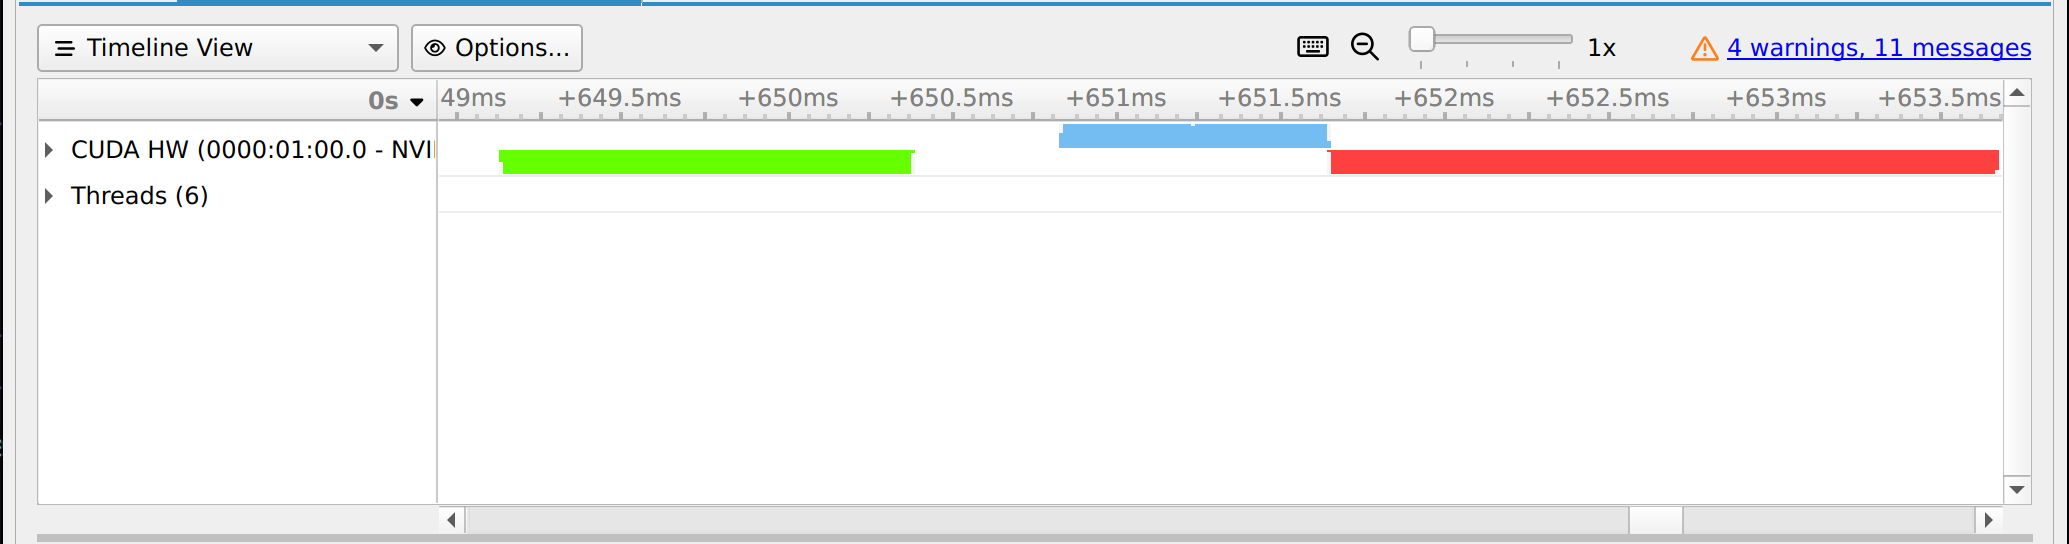
\includegraphics[width=120mm]{image/cuda_profile_non_stream.png}}
    \subfigure[Streamed kernel launch with shared memory.]{\label{fig:cuda_profile_stream}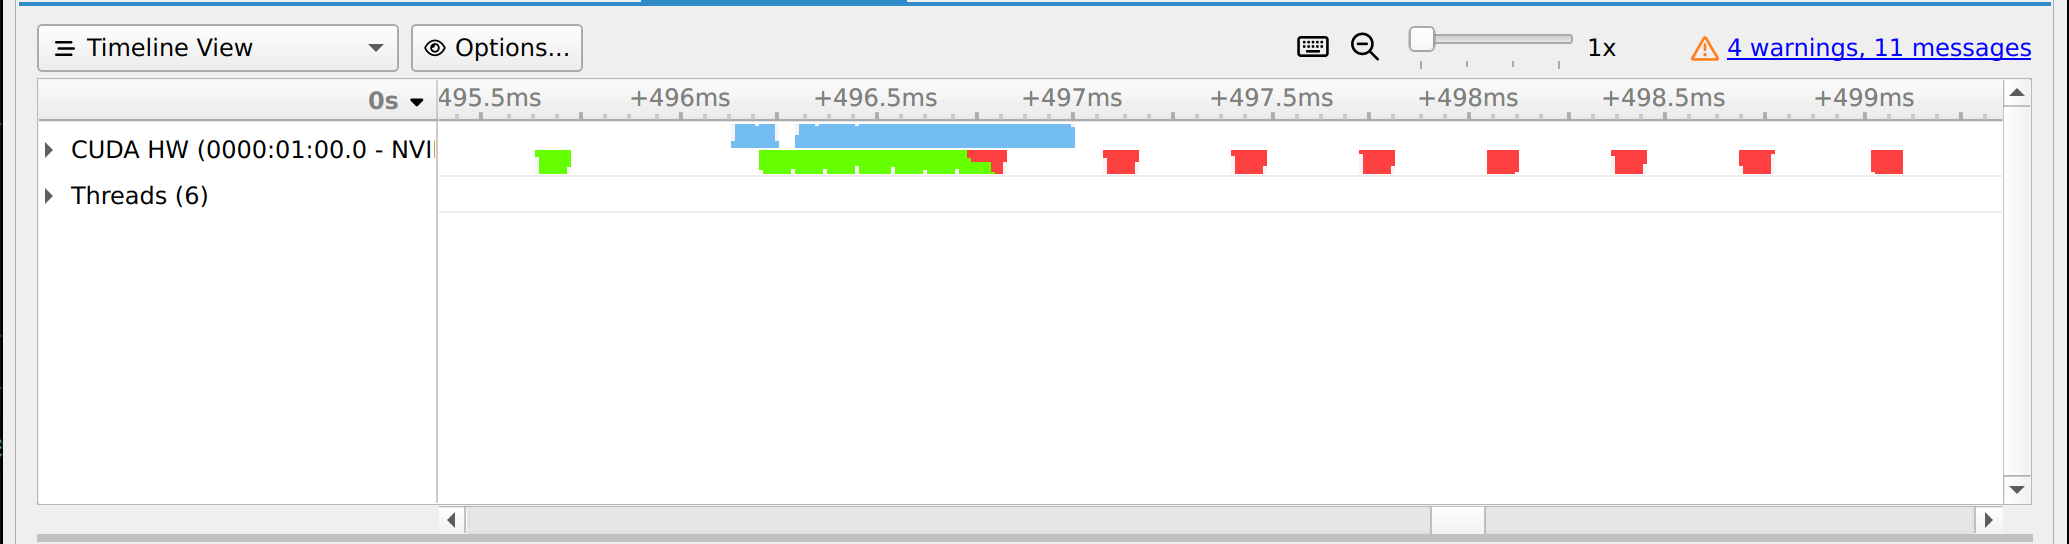
\includegraphics[width=120mm]{image/cuda_profile_stream.png}}
    \caption{An example of the improvement of streamed kernel launches and shared memory, shown using a profiler.}
    \label{fig:cuda_profile}
\end{figure}
